\section{Relays: One Circuit Controling Another Circuit}
\label{lab_relays}

%\makelabheader %(Space for student name, etc., defined in master.tex)

\bigskip

\begin{enumerate}[wide]

\item Find the relay in your kit, pictured below on the left.
This DPDT relay contains two electromagnetically controlled switches: one using pins 4, 6, and 8, and the other using pins 9, 11, and 13.  
%(Although there are only eight pins, the ``missing'' pins are still counted in the numbering.)  
When no power is applied to the magnetic coil (pins 1 and 16), the common terminal for each switch (pins 4 and 13) are connected to the ``normally closed'' terminals.  
But when you actuate the switch by applying 5~V across the coil, you will hear a little click, and each common terminal will be connected instead to that switch's ``normally open'' terminal.  
Use your DMM to figure out which of the remaining pins are the ``N.O.'' and ``N.C.'' terminals for each switch.  Copy the circuit diagram below on the right into your lab notebook, including pin numbers for both pairs of N.O. and N.C. terminals.
%(The dashed line in the circuit diagram indicates that the two switches always move together.  The two horizontal lines represent an iron core, like in a transformer, and are sometimes omitted.)

\begin{center}
\raisebox{0.5in}{
\includegraphics[scale=0.8]{relays/relay_picture.eps}}
\hspace{0.3in}
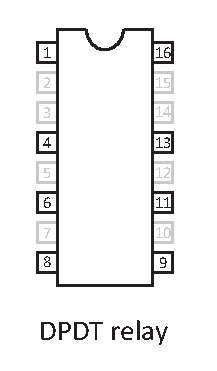
\includegraphics[scale=0.7]{relays/relay_pinout.eps}
\hspace{-0.1in}
{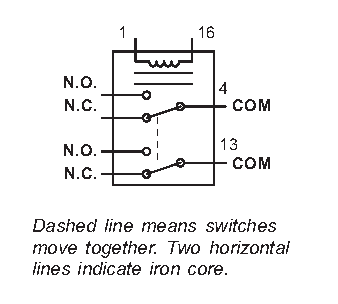
\includegraphics{relays/relay_diagram2.eps}}
\end{center}

\item The switches inside your relays can safely handle currents of about 1 Amp.  Slightly larger relays, perhaps one cubic inch in volume, can handle currents of 10 or 20 Amps.  By contrast, how large is the current in the coil of your relay?  (Measure it!  It should be a few tens of mA.)

%\item Use your 5~V power supply to actuate the relay, opening and closing a circuit that connects your function generator to your speaker.  Draw a good looking diagram of this circuit.

\item Build the circuit shown below, using your relay to open and close a connection between the 15~VDC power supply and a 10~k$\Omega$ load resistor.  
Turn the current to the coil on and off by literally touching two wires together.  
Use your oscilloscope to monitor both the voltage across the relay coil and the voltage across the 10~k$\Omega$ resistor, producing a graph similar to that on the right.  
How long is the delay $\Delta t$ between the time you apply 5~VDC to the coil and the time the N.O. contact closes?
(You should measure a few milliseconds.)

\begin{center}
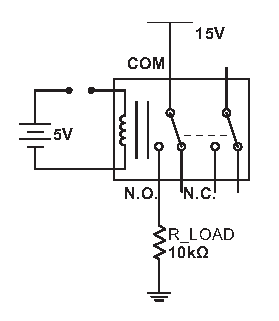
\includegraphics{relays/relay_timing_circuit.eps}
\hspace{0.6in}
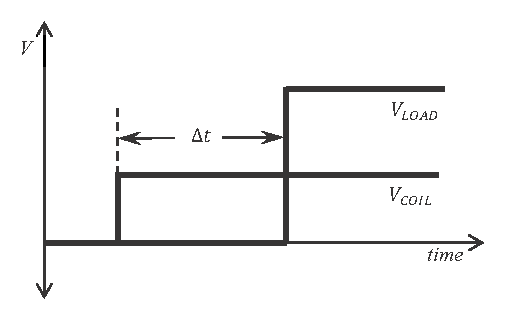
\includegraphics{relays/v_vs_t_graph.eps}
\end{center}

\item Change your circuit to measure how long it takes for the N.C. contact to open after applying 5~VDC to the coil.

\end{enumerate}

\textbf{Possible Exam Questions:}

\begin{itemize}

\item A digital ``AND'' gate is supposed to have a response time of 10 nanoseconds to any change in input.  Describe how you would use an oscilloscope to test this response time.  (How would you trigger, what coupling would you use, etc.) 

\end{itemize}







